\chapter{序論}

\par
対話システムは,発話解釈と発話生成の両方において発展を遂げており,我々の生活に浸透しつつある.しかし人間は,対話システムとの対話において不自然さやストレスを感じることも少なくない.本研究の目的は,人間に不自然さやストレスを与えることが無い,人間と長期的に共存可能な対話システムの実現である.

\par
対話システムと人間との対話では,対話システムが対話相手の心的状態を推定し,それを考慮した対話を行うことが重要である.
人間は,気分が落ち込んでいる対話相手の発話に対してネガティブな発話解釈をしたり,励ましの言葉をかけるように,対話相手の心的状態によって相手の発話の解釈を変えたり,自身の発話の内容を変えている.また,相手が知らないことについて詳しく説明したり,相手が好むことについて話を掘り下げる.対話システムにおいても,人間と同様に対話相手の心的状態に合わせて,発話解釈を変えたり,自身の発話の内容を変えることで,より自然でありストレスの少ない対話を実現することができる.つまり,対話相手に合わせた臨機応変な発話解釈や発話生成により対話における不自然さやストレスをなくすためには,対話相手の心的状態を推定することが必要となる.


\par
人間の心的状態を推定する研究には,人間の行動情報から心的状態を推定する研究や発話情報から心的状態を推定する研究が存在する.人間の行動情報から心的状態を推定する研究は,代表的には,環境の状態と環境中を移動する人間の行動や観測状況をベイズ推定\cite{alma9926464316904034}に適用し,環境中を移動する人間の信念と欲求を推定する研究 \cite{baker2011bayesian}があげられる.信念はどのようなことを考えているかということを意味し,欲求は何を望んでいるかということを意味する.発話情報から心的状態を推定する研究では,代表的には,発話から得られた事象を信念と捉え,考えられる欲求の候補を生成し,尤もらしい欲求を基に発話者の意図を推定する研究 \cite{高橋拓誠2015bdi}があげられる.また,心的状態を考慮することによる検索精度の向上のために検索クエリへの入力から人間の心的状態を推定する研究 \cite{10.1007/978-3-642-02481-8_4}や,学習効率の向上のために教師の発話から学習者の心的状態を推定する研究\cite{10.1007/978-3-319-40397-7_21}も存在する.

% 教師の発話から学習者の心的状態を推定する

\par
従来研究では,行動情報のみから人間の心的状態を推定する研究や発話情報のみから人間の心的状態を推定する研究は存在した.しかし,行動情報と発話情報の両方を活用し人間の心的状態を推定する研究はない.従来研究における心的状態の推定は,遠くから行動を観測している場合や立ち止まって対話をしている場合というように,行動情報のみが観測される場合や発話情報のみが観測される場合には有効である.しかし実世界では,行動情報と発話情報の両方が観測されることが多く,発話情報によって行動情報の解釈が変わったり,行動情報によって発話情報の解釈が変わることがある.
\begin{figure}[htbp]
  \begin{center}
    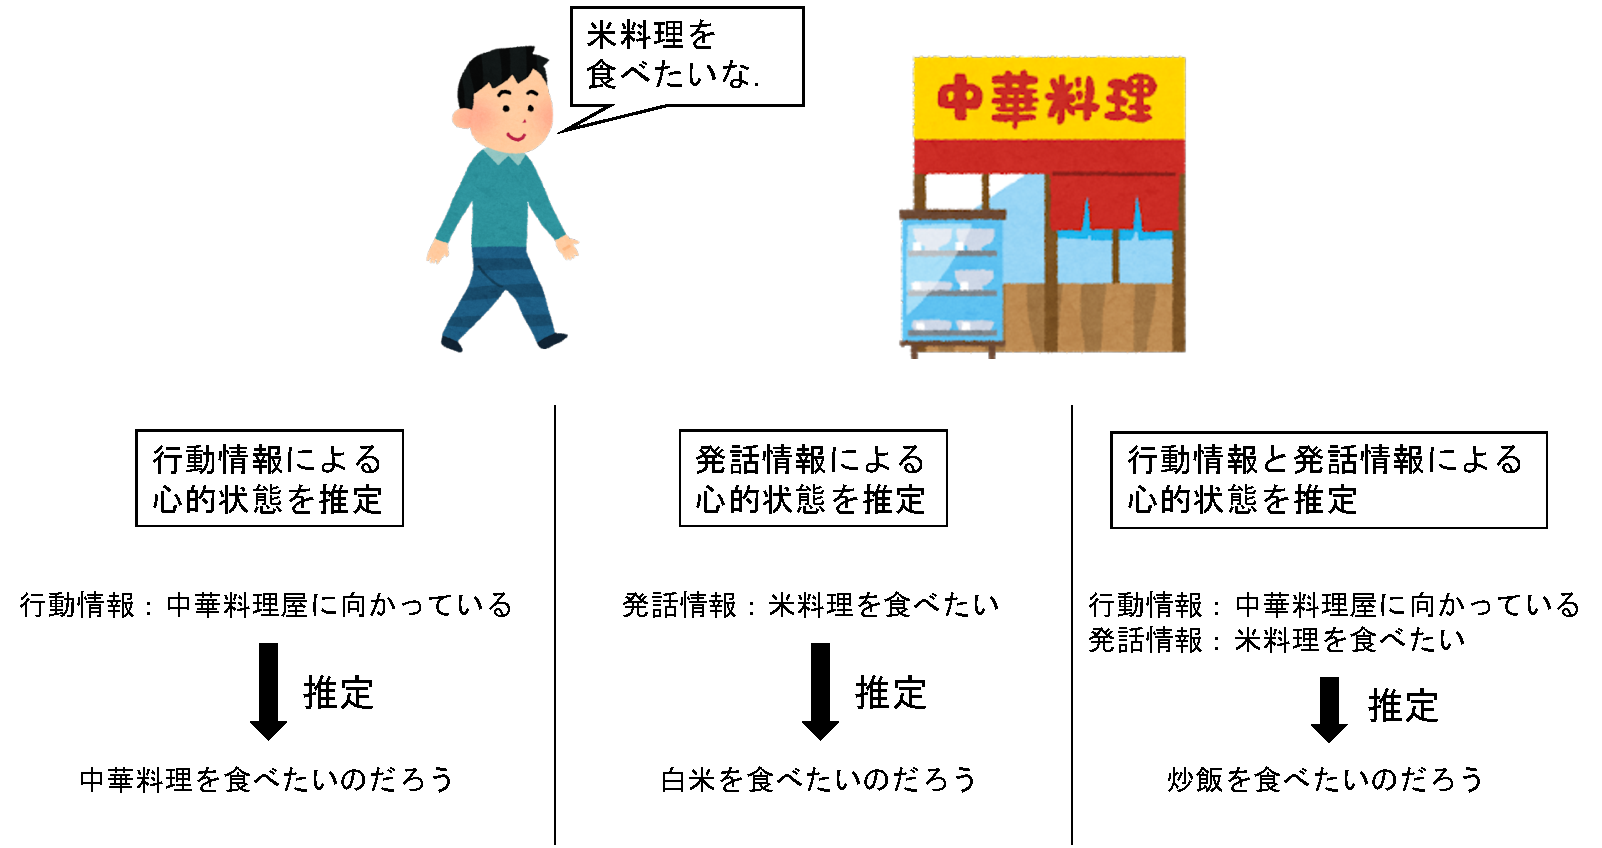
\includegraphics[scale=0.5]{./figure1.pdf}
    \caption{行動情報と発話情報の相互作用を考慮した心的状態の推定}
    \label{fig:fig1}
  \end{center}
\end{figure}
例えば,図\ref{fig:fig1}の左側の状況において,行動情報は「料亭と中華料理屋が並ぶ飲食店街に向かっている」と解釈できるが,図\ref{fig:fig1}の右側の状況のように「魚料理を食べたいな」という発話情報が観測された時,行動情報は「料亭に向かっている」という解釈に変わる.
従来研究では,行動情報と発話情報の両方が観測される場合においては,発話情報による行動情報の解釈の変化や,行動情報による発話情報の解釈の変化を捉えることが難しい.つまり,行動と発話の両方が観測される場合における従来研究における心的状態の推定では,行動と発話の相互作用の考慮による推定性能の向上の可能性が低いことが予想される.
% 従来研究では,行動情報のみから人間の心的状態を推定する研究や発話情報のみから人間の心的状態を推定する研究は存在した.しかし,行動情報と発話情報の両方を活用し人間の心的状態を推定する研究はない.従来研究における心的状態の推定は,遠くから行動を観測している場合や立ち止まって対話をしている場合というように,行動情報のみが観測される場合や発話情報のみが観測される場合には有効である.しかし実世界では,図\ref{fig:fig1}にように行動情報と発話情報の両方が観測されることが多く,発話情報によって行動情報の解釈が変わったり,行動情報によって発話情報の解釈が変わることがある.
% \begin{figure}[htbp]
%   \begin{center}
%     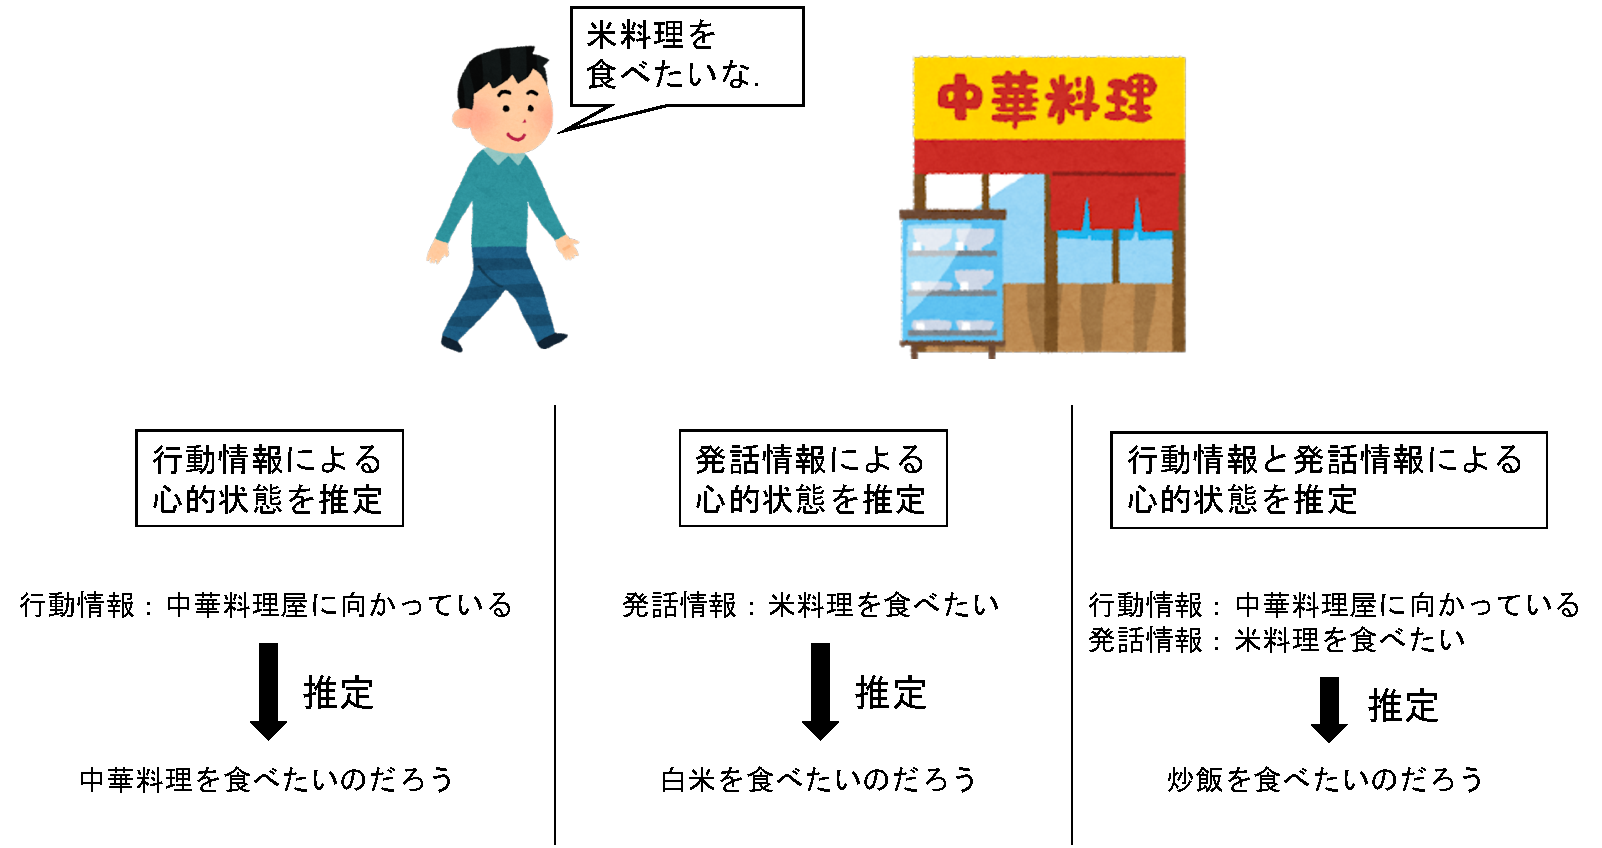
\includegraphics[scale=0.58]{./figure1.pdf}
%     \caption{心的状態の推定.人間が食事をとるために飲食店に向かう場面において,3通りの条件で心的状態を推定する.図の左側は,行動情報のみを活用して心的状態を推定した場合,図の中央は発話情報のみを活用して心的状態を推定した場合,図の右側は行動情報と発話情報の両方を活用して心的状態を推定した場合を表す.}
%     \label{fig:fig1}
%   \end{center}
% \end{figure}
% また行動情報のみを活用して「中華料理を食べたいのだろう」という心的状態を推定したり発話情報のみを活用して「白米を食べたいのだろう」という心的状態を推定するのに対し,行動情報と発話情報の両方を活用して「炒飯を食べたいのだろう」という心的状態を推定するように,行動情報と発話情報の両方を活用することにより,発話情報による行動情報の解釈の変化や行動情報による発話情報の解釈の変化を捉えることが可能となり,より多くの情報を基に推定を行うことができる.
% 従来研究では,行動情報と発話情報の両方が観測される場合においては,発話情報による行動情報の解釈の変化や,行動情報による発話情報の解釈の変化を捉えることが難しい.つまり,行動と発話の両方が観測される場合における従来研究における心的状態の推定では,行動と発話の相互作用の考慮による推定性能の向上の可能性が低いことが予想される.

\par
本研究では,行動情報と発話情報の両方から人間の心的状態の一部である信念および欲求を逐次的に推定するシステムMultimodal Inference of Mind SCAIN (MIoM SCAIN)を提案する.MIoM SCAINは,人間の信念および欲求の推定において,信念と欲求の組み合わせをを一つに断定するのではなく,同時に複数保持し,やり取りの中で動的に推定する.MIoM SCAINは,行動情報と発話情報の両方を推定に活用し,ベイズ推定によって人間の信念および欲求を逐次的に推定する.行動情報と発話情報の両方を推定に活用することにより,図\ref{fig:fig1}の右側の状況における推定のように,発話情報による行動情報の解釈の変化や行動情報による発話情報の変化を捉え,行動情報と発話情報の相互作用を考慮した推定が可能となる.実験では,独自で作成したデータセットを利用し,MIoM SCAINにより信念と欲求の推定を行い,行動情報と発話情報の両方を推定に活用することが有効であるかを評価する.

\par
本論文の構成は以下の通りである.第二章では,関連研究においてどのように人間の心的状態を推定していたかを述べる.第三章では,人間の行動情報と発話情報から信念と欲求を推定するシステムMIoM SCAINを提案する.第四章では,MIoM SCAINと単一の情報のみから信念と欲求を推定するシステムを用いて実験的に評価し,第五章では評価結果について考察する.第六章では,MIoM SCAINにおける今後の課題について述べる.最後に,第七章で本論文を締めくくる.
